% This is "sig-alternate.tex" V2.1 April 2013
% This file should be compiled with V2.5 of "sig-alternate.cls" May 2012
%
% This example file demonstrates the use of the 'sig-alternate.cls'
% V2.5 LaTeX2e document class file. It is for those submitting
% articles to ACM Conference Proceedings WHO DO NOT WISH TO
% STRICTLY ADHERE TO THE SIGS (PUBS-BOARD-ENDORSED) STYLE.
% The 'sig-alternate.cls' file will produce a similar-looking,
% albeit, 'tighter' paper resulting in, invariably, fewer pages.
%
% ----------------------------------------------------------------------------------------------------------------
% This .tex file (and associated .cls V2.5) produces:
%       1) The Permission Statement
%       2) The Conference (location) Info information
%       3) The Copyright Line with ACM data
%       4) NO page numbers
%
% as against the acm_proc_article-sp.cls file which
% DOES NOT produce 1) thru' 3) above.
%
% Using 'sig-alternate.cls' you have control, however, from within
% the source .tex file, over both the CopyrightYear
% (defaulted to 200X) and the ACM Copyright Data
% (defaulted to X-XXXXX-XX-X/XX/XX).
% e.g.
% \CopyrightYear{2007} will cause 2007 to appear in the copyright line.
% \crdata{0-12345-67-8/90/12} will cause 0-12345-67-8/90/12 to appear in the copyright line.
%
% ---------------------------------------------------------------------------------------------------------------
% This .tex source is an example which *does* use
% the .bib file (from which the .bbl file % is produced).
% REMEMBER HOWEVER: After having produced the .bbl file,
% and prior to final submission, you *NEED* to 'insert'
% your .bbl file into your source .tex file so as to provide
% ONE 'self-contained' source file.
%
% ================= IF YOU HAVE QUESTIONS =======================
% Questions regarding the SIGS styles, SIGS policies and
% procedures, Conferences etc. should be sent to
% Adrienne Griscti (griscti@acm.org)
%
% Technical questions _only_ to
% Gerald Murray (murray@hq.acm.org)
% ===============================================================
%
% For tracking purposes - this is V2.0 - May 2012

\documentclass{sig-alternate-05-2015}


\begin{document}

% Copyright
\setcopyright{acmcopyright}
%\setcopyright{acmlicensed}
%\setcopyright{rightsretained}
%\setcopyright{usgov}
%\setcopyright{usgovmixed}
%\setcopyright{cagov}
%\setcopyright{cagovmixed}


% DOI
\doi{10.475/123_4}

% ISBN
\isbn{123-4567-24-567/08/06}

%Conference
\conferenceinfo{PLDI '13}{June 16--19, 2013, Seattle, WA, USA}

\acmPrice{\$15.00}

%
% --- Author Metadata here ---
\conferenceinfo{WOODSTOCK}{'97 El Paso, Texas USA}
%\CopyrightYear{2007} % Allows default copyright year (20XX) to be over-ridden - IF NEED BE.
%\crdata{0-12345-67-8/90/01}  % Allows default copyright data (0-89791-88-6/97/05) to be over-ridden - IF NEED BE.
% --- End of Author Metadata ---

\title{Proposal of an Objective Metric for Hand Posture Comfort/Discomfort Evaluation.
\titlenote{(Produces the permission block, and
copyright information). For use with
SIG-ALTERNATE.CLS. Supported by ACM.}}
%\subtitle{[Extended Abstract]
%\titlenote{A full version of this paper is available as
%\textit{Author's Guide to Preparing ACM SIG Proceedings Using
%\LaTeX$2_\epsilon$\ and BibTeX} at
%\texttt{www.acm.org/eaddress.htm}}}
%
% You need the command \numberofauthors to handle the 'placement
% and alignment' of the authors beneath the title.
%
% For aesthetic reasons, we recommend 'three authors at a time'
% i.e. three 'name/affiliation blocks' be placed beneath the title.
%
% NOTE: You are NOT restricted in how many 'rows' of
% "name/affiliations" may appear. We just ask that you restrict
% the number of 'columns' to three.
%
% Because of the available 'opening page real-estate'
% we ask you to refrain from putting more than six authors
% (two rows with three columns) beneath the article title.
% More than six makes the first-page appear very cluttered indeed.
%
% Use the \alignauthor commands to handle the names
% and affiliations for an 'aesthetic maximum' of six authors.
% Add names, affiliations, addresses for
% the seventh etc. author(s) as the argument for the
% \additionalauthors command.
% These 'additional authors' will be output/set for you
% without further effort on your part as the last section in
% the body of your article BEFORE References or any Appendices.

\numberofauthors{8} %  in this sample file, there are a *total*
% of EIGHT authors. SIX appear on the 'first-page' (for formatting
% reasons) and the remaining two appear in the \additionalauthors section.
%
\author{
% You can go ahead and credit any number of authors here,
% e.g. one 'row of three' or two rows (consisting of one row of three
% and a second row of one, two or three).
%
% The command \alignauthor (no curly braces needed) should
% precede each author name, affiliation/snail-mail address and
% e-mail address. Additionally, tag each line of
% affiliation/address with \affaddr, and tag the
% e-mail address with \email.
%
% 1st. author
\alignauthor
Jonas A. Mayer
			%\titlenote{Dr.~Trovato insisted his name be first.}
	     \\
       \affaddr{Technische Universitaet Muenchen}\\
  %     \affaddr{1932 Wallamaloo Lane}\\
  %     \affaddr{Wallamaloo, New Zealand}\\
       \email{ga97qic@mytum.de}
% 2nd. author
\alignauthor
G.K.M. Tobin\\
       \affaddr{Institute for Clarity in Documentation}\\
       \affaddr{P.O. Box 1212}\\
       \affaddr{Dublin, Ohio 43017-6221}\\
       \email{webmaster@marysville-ohio.com}
% 3rd. author
\alignauthor Lars Th{\o}rv{\"a}ld\\
       \affaddr{The Th{\o}rv{\"a}ld Group}\\
       \affaddr{1 Th{\o}rv{\"a}ld Circle}\\
       \affaddr{Hekla, Iceland}\\
       \email{larst@affiliation.org}
}
% There's nothing stopping you putting the seventh, eighth, etc.
% author on the opening page (as the 'third row') but we ask,
% for aesthetic reasons that you place these 'additional authors'
% in the \additional authors block, viz.
% Just remember to make sure that the TOTAL number of authors
% is the number that will appear on the first page PLUS the
% number that will appear in the \additionalauthors section.

\maketitle
\begin{abstract}

TODO: Add Abstract

\end{abstract}


%
% The code below should be generated by the tool at
% http://dl.acm.org/ccs.cfm
% Please copy and paste the code instead of the example below. 
%
\begin{CCSXML}
<ccs2012>
<concept>
<concept_id>10003120.10003123.10011758</concept_id>
<concept_desc>Human-centered computing~Interaction design theory, concepts and paradigms</concept_desc>
<concept_significance>500</concept_significance>
</concept>
</ccs2012>
\end{CCSXML}

\ccsdesc[500]{Human-centered computing~Interaction design theory, concepts and paradigms}





%
% End generated code
%

%
%  Use this command to print the description
%
\printccsdesc

% We no longer use \terms command
%\terms{Theory}

\keywords{ACM proceedings; \LaTeX; text tagging}

\section{Introduction}

For a traditional desktop computer environment, there exist a number of different standardized interfaces for human-computer interaction using a mouse, keyboard and monitor, that allow the user to 
complete a variety of tasks effectively and efficiently by providing sets of shortcuts and macros. 

However, advancing technological progress as seen in virtual reality, augmented reality,
%not scientific
 robotics etc. open up new possibilities and create a need for new interaction techniques such as speech, gesture and posture interaction. 

In a human-robot interaction context, both speech as well as hand gestures and postures are common concepts. While speech interaction is struggling 
%not powerful, no need to talk all the time
with ambient noise, speech target identification and the creation of intuitive or learnable command sets, the main challenge for gestures and postures has been fighting physical forces that cause fatigue or discomfort and therefore limiting user experience as well as precision and performance as shown by Short \& Cauraugh \cite{short1999precision}.

%speech is not powerful enough
This paper is meant to support the creation and evaluation of hand posture catalogs for effective and efficient human-robot interaction by suggesting a hand posture comfort/discomfort metric, that allows for quick objective hand posture evaluation and demonstrating its effect on user performance. For this, state of the art comfort/discomfort models were applied to current hand anatomy and ergonomics knowledge to create models for hand comfort and discomfort. Using a large data set, gained in a user study, a machine learning algorithm generated a comfort/discomfort metric based on our model, which was verified in yet another user study. Finally another user study was used to show the the impact of comfort and discomfort, measured by our metric on performance in a pointing task.

We will first explain the theoretical basis of our comfort/discomfort model, before deriving our concrete metric from it. After that we will explain the methodology used for optimizing and validating the metric as well as present the results gained therefrom. Finally we will critically discuss ...
%overview over paper content
%concrete, important, scientific text


\section{Theoretical Foundation}
... is based on the comfort and discomfort models seen in Vink \& Hallbeck \cite{vink2012editorial}, defining comfort as a "pleasant state or relaxed feeling of a human being" mostly caused by subjective impressions and expectations and discomfort as "an unpleasant state of the human body" occurring from physical stress. Using this information and knowledge of the human hand anatomy, we broke down human hand comfort and discomfort in an non-resting (as opposed to resting on an object) hand into the following four components:

\subsection{Deviation from Range of Rest Posture}

%rest on supports
The \textbf{Range of Rest Posture (RRP)} as described in Apostolico et al. \cite{apostolico2014postural} is a range of angles for an articular joint, where the joint "can be considered statistically in rest", caused by muscle relaxation and therefore creating a maximum of comfort in this particular joint. In our case, we considered the human hand to have one RRP for each finger joint in a non-resting position with the palm facing downwards, resulting in a range of relaxed hand postures, similar to the one shown in Fig
%add figure
, where the comfort is maximized. 

As shown by Naddeo, Cappetti \& D'Oria 
\cite{naddeo2015proposal}, perceived comfort decreases for articular joints when deviating from the RRP and minimizes at the bounds of the natural range of motion. Applying this to the whole hand leads to the conclusion, that hand posture comfort can be evaluated by computing the total joint angle distance to the RRP.

\subsection{The Inter Finger Angles}

%hand anatomy
As it can be seen in figure X
%TODO: Add Figure
the hand has a very compact and highly connected system of muscles and tendons that limits the individual movement of fingers.
The fingers, excluding the thumb, share \textbf{most} of their flexor and extendor muscles, however minor individual flexion and extension of adjacent fingers is still possible due to finger tendons originating from different areas of the muscles. In the case of the \textit{Extensor digitorum communis} the finger tendons are even interconnected on the back of the hand. 

In conclusion of this, hand postures with high bending differences of adjacent fingers, again excluding the thumb, should lead to stress of tendons and muscles, as well as cognitive stress, minimizing comfort and increasing perceived discomfort.

\subsection{Finger Hyperextension}

As highlighted by LaViola \cite{laviola1999survey} hyperextension, as seen in Figure Y
%TODO: Add figure Y of Hyperextension
, "\textit{puts more strain on the }[metacarpophalangeal] \textit{joints and tendons than the hand is accustomed to}"\footnote{\cite{laviola1999survey}} and therefore causes discomfort. Even though this might seem redundant to the deviation from RRP on first sight, hyperextension takes a special position as it causes considerably more discomfort, compared to a full flexion of the fingers and compared to what the deviation from RRP would suggest.

\subsection{Finger Abduction}

Finger abduction, as seen in Figure Z,
%TODO: Add figure
also causes stress on the metacarpophalangeal joint, the interrosseus muscles and the tendons involved.

It was therefore also considered, analogue to the hyperextension, due to full abduction creating substantially more discomfort than full adduction.


\section{Hand Posture Comfort/Discomfort Metric}
%Hand Model!! Angle Based Hand Model/ X-DOF
For the computation of our metric we used an angle based hand model as described by Su \& Futura \cite{su1994logical}, as it made extraction of angles pretty trivial. Instead of the full 23 degrees of freedom, described by LaViola \cite{laviola1999survey}, we used that simplified model that neglects the metacarpocarpal joint of the fourth and fifth digit. This was for one due to the \textbf{Leap} using the same model for detecting hands and for another due to the metacarpocarpal joint not being noticeable to influence hand postures at all.

The 21 DOF angle based hand model was then simply handled as a float vector of length 21. 
%TODO: get a real explanation

\subsection{Comfort Metric}

The only component of our theoretical model to display comfort is the deviation of the RRP. In our implementation the RRP was represented by a set of 50 relaxed hand postures recorded with the Leap. The metric was simply computed by calculating the minimum euclidean distance to the our RRP set, initially for the whole hand.
The resulting comfort metric value would grow indirectly proportional to the expected perceived comfort, with a value of 0 describing the maximum amount of comfort. 


\subsection{Discomfort Metric}

Our discomfort metric consists of three components: inter finger angles, hyper extension and abduction. These components were computed individually, multiplied by weight coefficients and finally added. Note that our discomfort metric did not involve knowledge of the thumb.

The inter finger angle component was computed by first summing up the flexion/extension angles of metacarpophalangeal (MCP), proximal interphalangeal (PIP) and distal interphalangeal (DIP) joints for each finger and adding up the differences in total bending of adjacent fingers (3 values). 

For the hyper extension component we simply summed up the the flexion/extension angle of the fingers MCP that had a negative angle and were therefore hyperextended.

We computed the abduction component by adding up the absolute adbduction/adduction angle for the finger, based on fact, that in our model a fully adducted finger has an adbduction angle of 0.

The resulting discomfort metric value is expected to grow proportionally with the perceived discomfort, with a value of 0 indicating the minimum discomfort. 

\subsection{Improvement of the Naive Metric}

Even though the naive metrics contain the causes for comfort and discomfort, that we identified in hands and probably would already suffice to get a coarse overview over the comfort and discomfort of a hand posture, it still lacks consideration for the anatomical differences between the fingers. The importance of this differentiation can be seen in when extending a the index finger from a closed fist as opposed to extending the ring finger. 
The concept of improvement for this is trivial: instead of applying the metrics to the whole hand, have a look at the contributions from the individual fingers and weight them with importance coefficients. 

In our case we have 5 comfort values and a total of 12 discomfort values. However, the exact weighting coefficients are generally unknown. To solve this problem, we reduced it to a curve fitting problem with 17 unknowns and used data, obtained from user evaluations to find the correct coefficients.

\section{Methodology}

For the collection of data, we created a test environment using Unity 3D with a total of two tasks. In the fist task, the user would be shown a randomly generated hand posture on screen, using our naive metric to ensure a somehow homogenous distribution of expected comfort and discomfort. The participant was asked to mimic the hand posture with his or her dominant hand and afterward rate the hand. As we did not expect the subjects to be familiar with current comfort and discomfort models, we asked them to rate hand postures on intuitive scale ranging from 10 (very comfortable) to 0 (very uncomfortable). The user was told to rate the hand posture with 0 points if he or she was unable to reproduce it. Before the actual evaluation the users were shown two hand postures to get a reference. The first hand posture was a completely relaxed hand, the second hand posture was a randomly generated hand, that was impossible to mimic.

In the second task, the participant was again given a randomly generated hand posture. Again the user had to mimic the hand posture with his dominant hand and give it a rating from 0 to 10. After confirming his or her rating, the subject had to perform a target shooting task. Therefore we tracked the palm of the participant's hand using an ART Hand Tracking Device, giving the user a minimalistic representation of their palm position and indicating the forward direction of the palm with a rendered ray. The subject had to use this ray to aim down a total of 12 targets, appearing in random order, and shoot them, by pressing a button. By recording the hand posture before the trial using a Leap, and checking the the hand posture during the test, we made sure that the user would not brake the posture during the test. 

As a metric for precision and performance, we measured the total time taken for the test. In order to have this affected by precision, we made the targets rather small and told the participants to minimize the time taken.

We conducted a total of two user studies involving 21 voluntary participants, that gained us 250 and 60 data sets for the metric and one study gaining us 35 data sets for the target shooting. The subjects were compensated with refreshments and/or sweets.
The participants were were informed over the aim of the study as well as their specific objectives beforehand.

As we expected both comfort and discomfort to affect performance and due to the users only giving us one value for comfort and discomfort, we decided to combine comfort and discomfort in our model as well. As the finding of the best fitting coefficients can be reduced to a curve fitting problem, we used the least squares algorithm on the first 250 data sets to solve the problem. We then tested our results against the remaining 60 data sets to check them for correctness. 

\section{Results \& Discussion}

The results of our study are shown in Figure \ref{fig:trainingData} to \ref{fig:targetShooting}, with the dots representing the discrete samples and the line showing the smoothed conditional mean, calculated by the \texttt{geom\_smooth}function in R with standard parameters. The respective Pearson correlation coefficients and p-values can be taken from Table \ref{tab:correlations}.

Unsurprisingly, there was a correlation in the training data between the user rating and our refined metric generated by this data as it can be seen in Figure \ref{fig:trainingData}. 


\begin{figure}
\centering
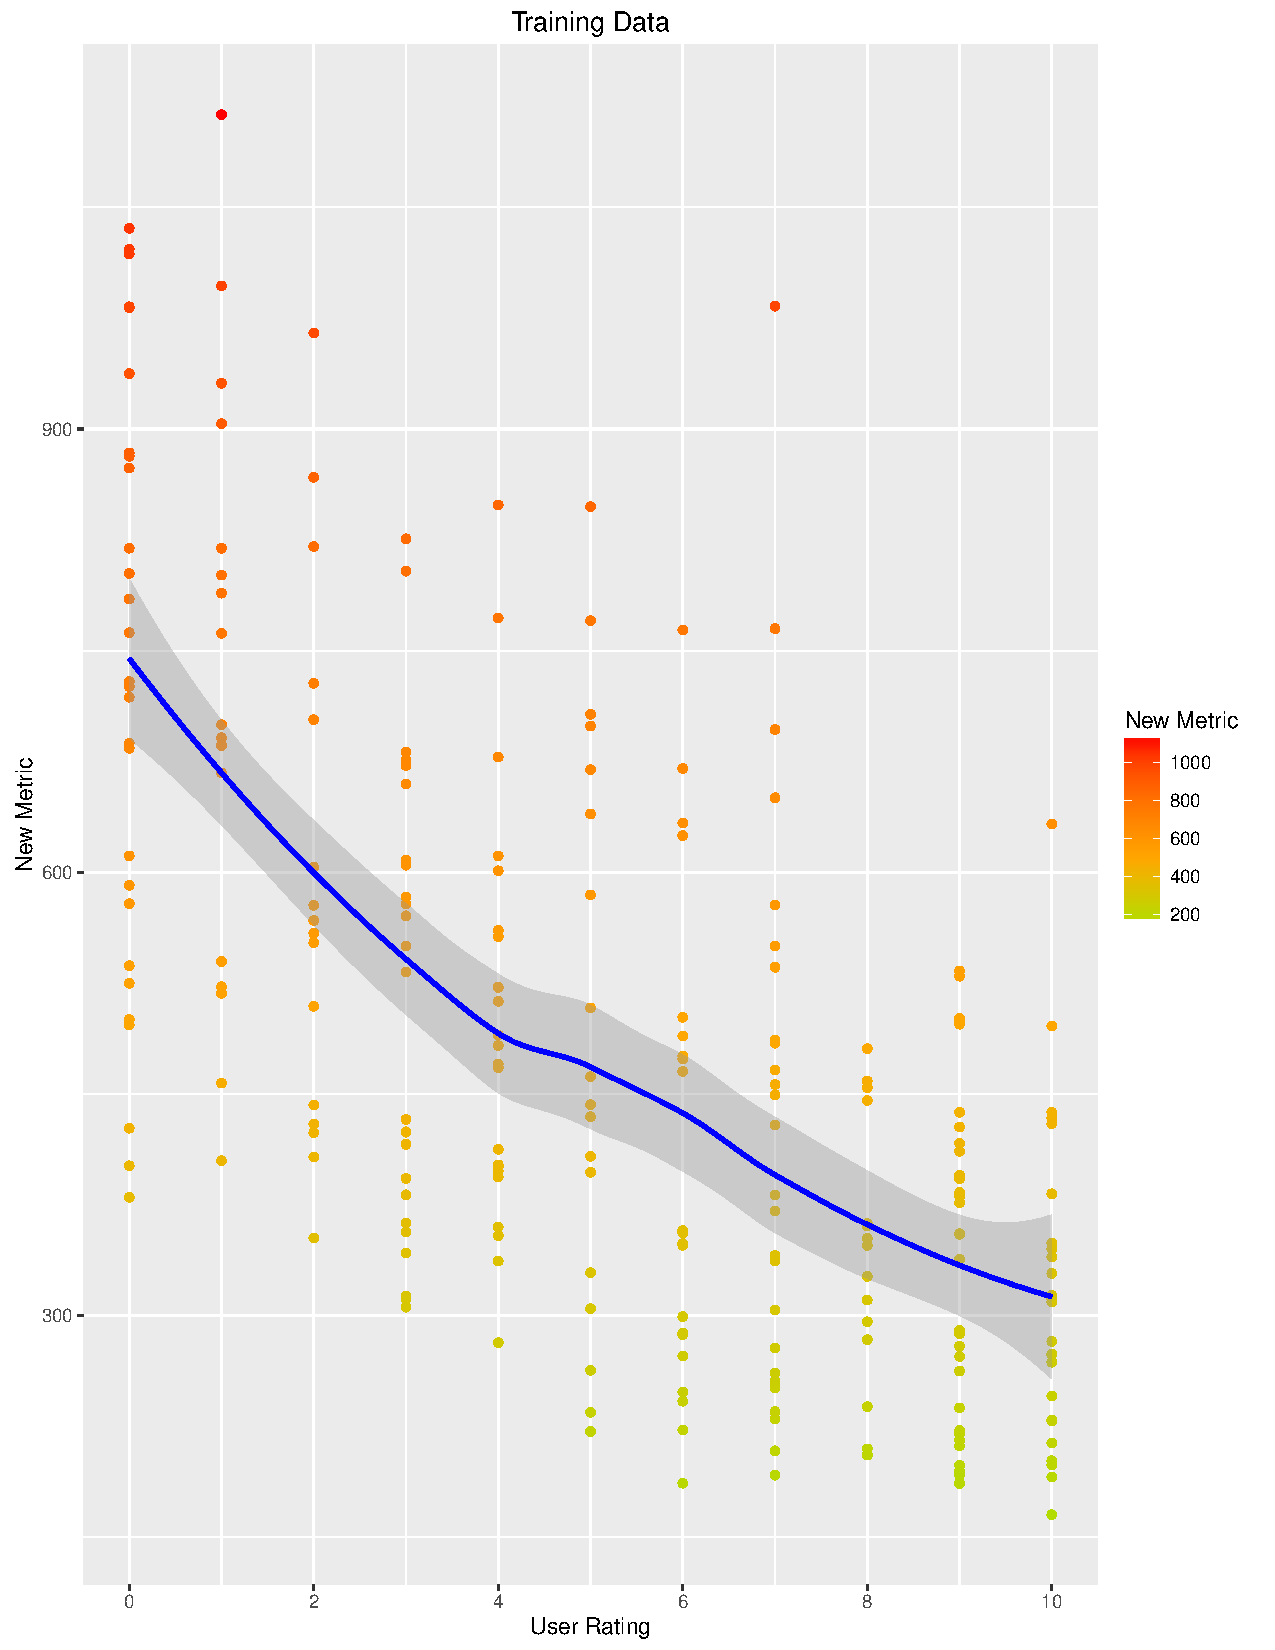
\includegraphics[width=8.45cm]{TrainingData}
\vspace{-20pt}
\caption{Correlation in Training Data between User Rating and Computed Metric Value}
\label{fig:trainingData}
\vspace{-10pt}
\end{figure}

\begin{figure}
\centering
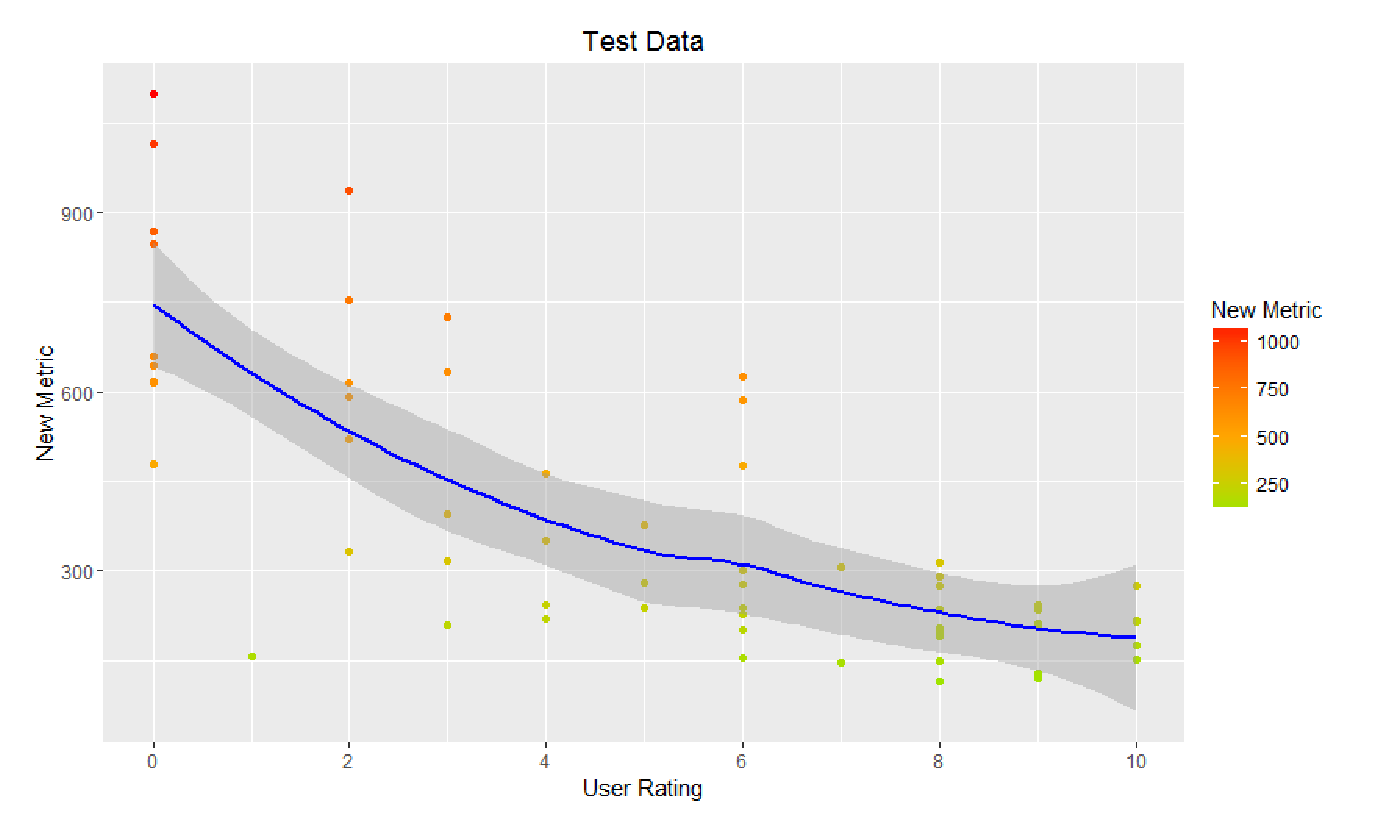
\includegraphics[width=8.45cm]{TestData}
\vspace{-20pt}
\caption{Correlation in Test Data between User Rating and Computed Metric Value}
\vspace{-10pt}
\label{fig:testData}
\end{figure}

\begin{figure}
\centering
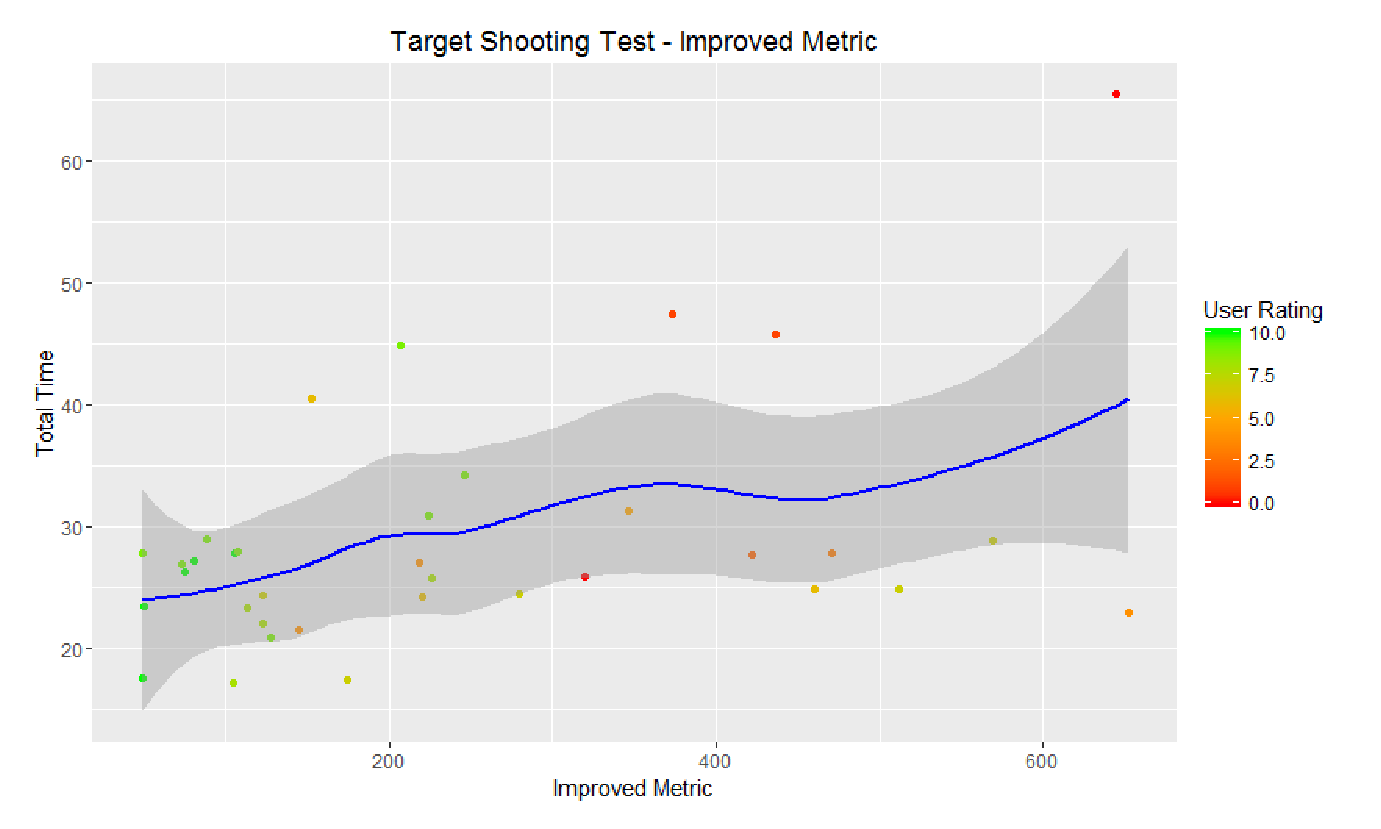
\includegraphics[width=8.45cm]{TargetShooting}
\vspace{-20pt}
\caption{Correlation between Computed Metric Value and Total Time in Target Shooting}
\label{fig:targetShooting}
\vspace{-10pt}
\end{figure}

\begin{table}
\centering
\begin{tabular}{|c|c|c|} \hline
\#Figure & Correlation & p-value\\ \hline
\ref{fig:trainingData} & -0.6453242 & < 2.2e-16\\ \hline
\ref{fig:testData} & -0.748993 & 5.89e-12\\ \hline
\ref{fig:targetShooting} & 0.4236101 & 0.01122\\ \hline
\end{tabular}
\caption{Frequency of Special Characters}
\label{tab:correlations}
\end{table}

%\end{document}  % This is where a 'short' article might terminate

%
% The following two commands are all you need in the
% initial runs of your .tex file to
% produce the bibliography for the citations in your paper.
\bibliographystyle{abbrv}
\bibliography{handComfort}  % sigproc.bib is the name of the Bibliography in this case
% You must have a proper ".bib" file
%  and remember to run:
% latex bibtex latex latex
% to resolve all references
%
% ACM needs 'a single self-contained file'!
%
%APPENDICES are optional
%\balancecolumns

%\balancecolumns % GM June 2007
% That's all folks!
\end{document}
